\documentclass[conference]{IEEEtran}

\usepackage{amsmath,amssymb}
\usepackage{graphicx}
\usepackage{textcomp}
\usepackage{booktabs}
\usepackage[sort,compress]{cite}
\usepackage{url}
\usepackage[font=footnotesize,labelfont=bf,skip=2pt]{caption}

\setlength{\textfloatsep}{3pt plus 1pt minus 1pt}
\setlength{\floatsep}{2pt plus 1pt minus 1pt}
\setlength{\intextsep}{3pt plus 1pt minus 1pt}
\setlength{\dblfloatsep}{3pt plus 1pt minus 1pt}
\setlength{\dbltextfloatsep}{3pt plus 1pt minus 1pt}
\setlength{\abovedisplayskip}{3pt plus 1pt minus 1pt}
\setlength{\belowdisplayskip}{3pt plus 1pt minus 1pt}

\makeatletter
\let\oldthebibliography\thebibliography
\let\endoldthebibliography\endthebibliography
\renewenvironment{thebibliography}[1]{%
  \oldthebibliography{#1}%
  \scriptsize
  \setlength{\itemsep}{0pt}%
  \setlength{\parsep}{0pt}%
  \setlength{\parskip}{0pt}%
}{\endoldthebibliography}
\makeatother

\graphicspath{{figs/}}

\def\BibTeX{{\rm B\kern-.05em{\sc i\kern-.025em b}\kern-.08em
    T\kern-.1667em\lower.7ex\hbox{E}\kern-.125emX}}

\begin{document}

\title{Monte Carlo Reliability Sizing of PV--Hydrogen Backup for Data-Centre Energy-Internet Nodes}

% NOTE TO AUTHOR: please verify/complete affiliation, city/country and
% e-mail address below before submission.
\author{
\IEEEauthorblockN{Rahul Rajeevkumar Urs}
\IEEEauthorblockA{
Khalifa University\\
Abu Dhabi, United Arab Emirates\\
rahul.urs@ku.ac.ae}
}

\maketitle

\begin{abstract}
Data centres are emerging as controllable Energy-Internet nodes, yet renewable-integration studies often separate grid-connected cost/carbon optimisation from outage backup. This paper presents a reliability-constrained sizing framework for a photovoltaic (PV)--electrolyser--fuel cell--hydrogen storage--grid microgrid serving a 24/7 data centre, with an existing N+1 diesel genset retained as the backstop for any residual outage energy. Hourly grid-connected dispatch is run to hydrogen-inventory steady state and coupled to a 5000-event Monte Carlo outage assessment. For a 5~MW critical-IT data centre in Abu Dhabi, the lowest-cost design with zero unmet energy across the sampled outages uses 22~MW PV, a 10~MW electrolyser, a 5~MW fuel cell and a 17{,}102~kg (57-hour) H$_2$ tank; it attains $P_{\mathrm{survive}}=1.000$ over the sampled events and an LCOE of 0.1272~\$~kWh\textsuperscript{-1}. Relative to a grid-plus-diesel baseline serving the same load and design-basis outage energy, this design cuts annual CO\textsubscript{2} emissions by 44.5\% at a 52.8\% cost increase, equivalent to \$233.6~tCO\textsubscript{2}\textsuperscript{-1}. The central result is structural: unlike a diurnally cycling, power-rate-limited battery, the H$_2$ tank fills opportunistically over the year, so outage survival rises monotonically with autonomy until the sampled outage draw is covered.
\end{abstract}

\begin{IEEEkeywords}
Energy Internet, data centres, photovoltaic power systems, hydrogen storage, electrolysers, fuel cells, diesel generators, reliability, techno-economic analysis, Monte Carlo methods.
\end{IEEEkeywords}

\begin{table}[!b]
\centering
\caption{Nomenclature}
\label{tab:nomenclature}
\scriptsize
\setlength{\tabcolsep}{2pt}
\begin{tabular}{@{}p{0.24\columnwidth}p{0.70\columnwidth}@{}}
\toprule
Symbol & Meaning \\
\midrule
$P_{PV}(t)$, $P_{load}(t)$ & PV generation and facility load [MW] \\
$P_{EZ}$, $P_{FC}$ & Electrolyser and fuel-cell ratings [MW] \\
$m_{H_2}$, $a$ & Usable H$_2$ capacity [kg]; FC autonomy [h] \\
$s$, $\eta_{FC}$ & Electrolyser specific energy [kWh kg$^{-1}$]; FC efficiency \\
$\mathrm{LHV}_{H_2}$ & Hydrogen lower heating value [kWh kg$^{-1}$] \\
$u^{(i)}$ & Unmet energy in outage event $i$ [MWh] \\
$P_{\mathrm{survive}}$ & Share of outages fully served by PV+H$_2$ \\
$\mathrm{EUE}_{\mathrm{yr}}$ & Expected unserved energy [MWh yr$^{-1}$] \\
$f_E$, CFE & Outage-energy and carbon-free-energy fractions \\
\bottomrule
\end{tabular}
\end{table}

\section{Introduction}

Global electricity demand from data centres, artificial intelligence and cryptocurrency was estimated at 460~TWh in 2022 and could reach 620--1050~TWh by 2026 \cite{iea2024,figini2025}. Because many data centres can host local generation, storage and controllable backup, they are natural ``cell-level'' Energy-Internet nodes \cite{dong2024}.

Reliability remains the dominant constraint. Power remains the leading cause of impactful outages \cite{uptime2026}, while conventional resilience is still mainly provided by diesel generator sets. Hydrogen produced from PV surplus, stored on site, and reconverted through a fuel cell has therefore become a candidate long-duration, diesel-displacing backup pathway. A 1.5~MW proton-exchange-membrane (PEM) fuel cell has already supported a Microsoft data-centre backup demonstration over a simulated 48-hour event \cite{catmsft2024}, and techno-economic studies now examine fuel-cell-powered and hybrid electrolyser--fuel-cell data-centre concepts \cite{kurtz2023,ai2026}.

Existing work covers renewable/hydrogen sizing in power networks \cite{kayacik2024} and data-centre fuel-cell economics \cite{kurtz2023}. However, it has not jointly examined a Monte Carlo outage-survival metric, a retained diesel backstop representative of retrofit practice, and a storage-autonomy sweep that reveals whether reliability saturates before all sampled outage energy is covered.

The work contributes a steady-state PV--H$_2$ dispatch model, Numba-compiled outage Monte Carlo kernels \cite{lam2015numba}, a refined 2409-configuration Abu Dhabi sizing sweep, and a diesel-retained baseline comparison. The main finding is that hydrogen survival does not exhibit the sub-unity saturation seen in a companion battery-only case: additional autonomy keeps improving survival until the sampled outage energy is covered.

\section{System Architecture and Case Study}

\begin{figure*}[!t]
\centering
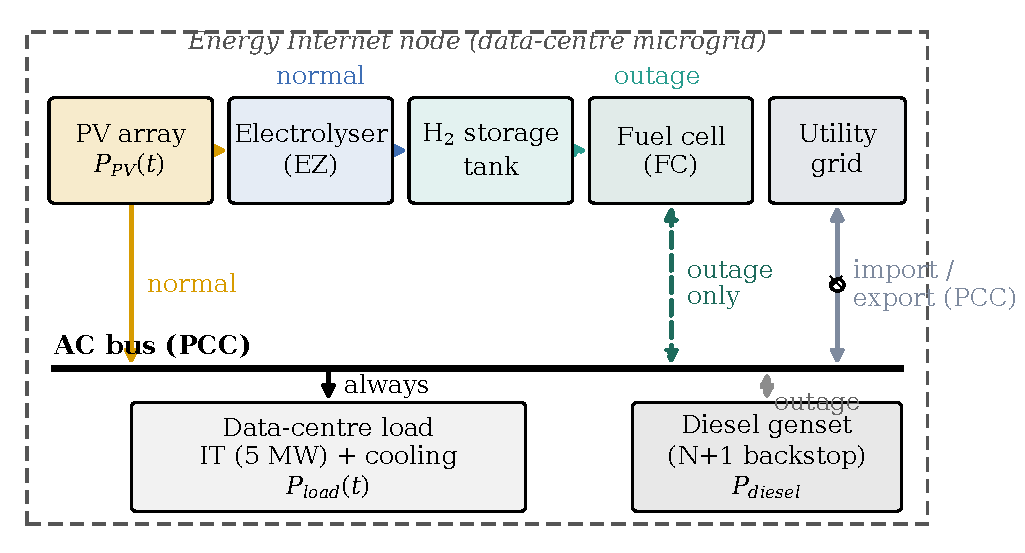
\includegraphics[width=\textwidth]{fig1_architecture.pdf}
\caption{System architecture: PV array, electrolyser (EZ), hydrogen storage tank, fuel cell (FC) and the utility grid connect to a common AC bus serving the data-centre's critical-IT and cooling load. Solid arrows denote normal grid-connected energy flows (PV surplus charges the tank via the electrolyser); dashed arrows denote outage-only flows (the fuel cell discharges the tank; the N+1 diesel genset covers any residual deficit).}
\label{fig:architecture}
\end{figure*}

The PV-hydrogen architecture in Fig.~\ref{fig:architecture} is represented as an Energy-Internet node. A PV array, an electrolyser-tank-fuel cell hydrogen chain, and the utility grid connect to a common AC bus at the point of common coupling (PCC) serving the data-centre's critical-IT and cooling load. An existing N+1 diesel genset -- sized to the critical-IT load with one redundant unit -- shares the same bus but is dispatched only when the site is islanded, covering whatever residual deficit PV+H\textsubscript{2} cannot meet (Section~III).

The case-study site is identical to a companion PV-battery study: a 5~MW critical-IT data centre in Abu Dhabi, UAE (24.45$^\circ$N, 54.37$^\circ$E), with total facility load obtained from the critical-IT load via the same ambient-temperature-dependent power usage effectiveness (PUE) relation,
\begin{equation}
\mathrm{PUE}(T_{amb}) = 1.20 + 0.010\;^{\circ}\mathrm{C}^{-1}\max(0,\, T_{amb} - 25^{\circ}\mathrm{C}),
\label{eq:pue}
\end{equation}
adopted as a representative, parameterised assumption rather than a site-measured curve, giving an annual mean PUE of 1.244, a mean total load of 6.224~MW (range 5.70--7.15~MW) and an annual energy demand of 54{,}520~MWh. Table~\ref{tab:system} summarises the case-study parameters and the sizing-sweep grid.

\begin{table}[t]
\centering
\caption{Case-Study System and Sizing-Sweep Parameters}
\label{tab:system}
\scriptsize
\begin{tabular}{@{}p{0.42\columnwidth}p{0.53\columnwidth}@{}}
\toprule
Parameter & Value \\
\midrule
Location & Abu Dhabi, UAE (24.45$^\circ$N, 54.37$^\circ$E) \\
Critical-IT load & 5~MW \\
PUE & Eq.~(\ref{eq:pue}); mean 1.244 \\
PV tilt / orientation & 24$^\circ$ / south \\
Electrolyser rating & 10~MW if autonomy $>0$ \\
Fuel-cell rating & 5~MW if autonomy $>0$ \\
Diesel genset rating & 10~MW (N+1) \\
Outage design frequency & 2 events yr$^{-1}$ \\
Outage duration (60\%) & $U(0.25, 2)$~h \\
Outage duration (30\%) & $U(2, 12)$~h \\
Outage duration (10\%) & $U(12, 96)$~h \\
Outage MC trials per design & 5000 \\
Sweep: PV capacity & 8--24~MW (0.5~MW steps, 33 levels) \\
Sweep: H$_2$ autonomy & 0--72~h (1~h steps, 73 levels) \\
Total configurations & $33\times73=2409$ \\
\bottomrule
\end{tabular}
\end{table}

\section{Methodology}

\subsection{Resource and Load Model}

Hourly plane-of-array irradiance is synthesised from a clearness-index distribution (Beta(9.0, 3.2)), the Erbs diffuse-fraction correlation \cite{erbs1982}, and isotropic-sky transposition \cite{duffie2013}. A NOCT temperature model with a $-0.35\%\,^{\circ}\mathrm{C}^{-1}$ coefficient gives 2252.1~kWh~m$^{-2}$ annual GHI, 2387.4~kWh~m$^{-2}$ plane-of-array irradiance, and 23.08\% mean PV capacity factor. Ambient temperature spans 7.4--45.3$^{\circ}$C; total facility load follows Eq.~(\ref{eq:pue}).

\subsection{Dispatch Model}

\emph{Normal (grid-connected) mode.} At hour $t$, let $\mathrm{net}(t) = P_{PV}(t)-P_{load}(t)$. If $\mathrm{net}(t)\ge0$, the electrolyser charges the tank at $\min(\mathrm{net}(t),P_{EZ},\mathrm{room}(t)s/1000)$, where $s=57$~kWh~kg$^{-1}$; further surplus is exported. If $\mathrm{net}(t)<0$, the deficit is imported from the grid. The fuel cell is not dispatched in normal operation because the electrolyser--fuel-cell round trip is only about 30\%; the tank is reserved for outages.

Because the tank only charges in normal mode, a single annual pass from empty contains a fill transient rather than a repeating cycle. We therefore repeat $\texttt{normal\_dispatch()}$, carrying the year-end inventory forward until its change is below $10^{-6}$~kg (at most 16 passes). The converged trajectory, full at steady state for every nonzero-autonomy case, initialises the outage Monte Carlo.

\emph{Outage (islanded) mode.} On a grid outage, load is shed to the 5~MW critical-IT demand. PV serves this load first; surplus is curtailed because islanded electrolyser operation is excluded. Any deficit is supplied by the fuel cell from the hydrogen inventory at the outage start, and residual unmet energy is recorded and assigned to the retained N+1 diesel genset (Section~\ref{sec:techno}).

Both the normal-mode dispatch and the outage Monte Carlo are implemented as explicit-loop kernels compiled with Numba's just-in-time (JIT) compiler \cite{lam2015numba}. The full 2409-configuration sizing sweep (Section~\ref{sec:sweep}), each evaluated against 5000 outage draws, executes in a few seconds on the local runtime.

\subsection{Reliability Metric}

For each sizing, $N=5000$ outage events $(t_0^{(i)}, d^{(i)})$ are drawn from a shared set of start hours and durations: 60\% transient, $U(0.25,2)$~h; 30\% medium, $U(2,12)$~h; and 10\% extended, $U(12,96)$~h. Each event is simulated in islanded mode from the steady-state hydrogen inventory at $t_0^{(i)}$, yielding unmet energy $u^{(i)}$. The empirical Outage Survival Probability is
\begin{equation}
P_{\mathrm{survive}} = \frac{1}{N}\sum_{i=1}^{N} \mathbb{1}\!\left[u^{(i)} \le \varepsilon\right],
\label{eq:psurvive}
\end{equation}
i.e.\ the fraction of events fully served by PV+H\textsubscript{2} alone ($\varepsilon=10^{-9}$~MWh). A complementary energy-coverage fraction,
\begin{equation}
f_E = 1 - \frac{\mathrm{EUE}_{\mathrm{yr}}}{E_{\mathrm{outage,total}}},
\qquad
\mathrm{EUE}_{\mathrm{yr}} = \overline{u}\cdot f_{\mathrm{outage}},
\label{eq:fE}
\end{equation}
expresses the share of the design-basis annual outage energy $E_{\mathrm{outage,total}}$ (Section~\ref{sec:results-e}) that PV+H\textsubscript{2} displaces from the diesel genset in aggregate, where $\overline{u}$ is the mean unmet energy per event and $f_{\mathrm{outage}}=2$~events~yr$^{-1}$ is the design-basis outage frequency (Table~\ref{tab:system}).

\subsection{Techno-Economic Model}
\label{sec:techno}

Component capital costs are annualised via the capital recovery factor,
\begin{equation}
\mathrm{CRF}(r,n) = \frac{r(1+r)^n}{(1+r)^n - 1},
\label{eq:crf}
\end{equation}
applied at $r=7\%$ over each component's own economic lifetime $n$ (Table~\ref{tab:costs}). A hydrogen-autonomy target $a$ [h] is converted to a required tank capacity via
\begin{equation}
m_{H_2} = \frac{a \cdot P_{FC}\cdot 1000}{\eta_{FC}\cdot\mathrm{LHV}_{H_2}}\;\;[\mathrm{kg}],
\label{eq:h2mass}
\end{equation}
where $P_{FC}$ is the fuel cell power rating [MW], $\eta_{FC}=0.50$ and $\mathrm{LHV}_{H_2}=33.33$~kWh~kg$^{-1}$. PV capex/lifetime follow NREL's 2024 ATB \cite{nrelatb2024}. The electrolyser capex is set to \$1{,}250~kW$^{-1}$ as a cost-down scenario; DOE Record \#24005 provides the 57~kWh~kg$^{-1}$ PEM specific energy and reports a higher current installed-cost range \cite{doe24005}. Fuel-cell and storage assumptions follow the literature ranges in \cite{kayacik2024}. Grid prices (\$0.080/\$0.030~kWh$^{-1}$) are scenario values benchmarked to published Abu Dhabi tariffs \cite{rsbtariffs}; grid carbon intensity is 0.450~kg~kWh$^{-1}$, above the UAE 2030 target of 0.27~kg~kWh$^{-1}$ \cite{uaees2050}. Annualised system cost sums capex, fixed O\&M and net grid exchange; dividing by annual demand gives LCOE. The carbon-free-energy fraction is
\begin{equation}
\mathrm{CFE} = 1 - \frac{E_{\mathrm{grid,import}}}{E_{\mathrm{load}}}.
\label{eq:cfe}
\end{equation}

\begin{table}[t]
\centering
\caption{Techno-Economic Parameters}
\label{tab:costs}
\scriptsize
\begin{tabular}{@{}lll@{}}
\toprule
Component & Parameter & Value \\
\midrule
PV & CAPEX & \$750~kW$^{-1}$ \\
 & Life / FOM & 25~yr / 1.5\% \\
EZ (PEM) & CAPEX & \$1{,}250~kW$^{-1}$ \\
 & Life / FOM & 20~yr / 2.5\% \\
 & Specific energy & 57~kWh~kg$^{-1}$ \\
FC (PEM) & CAPEX & \$1{,}200~kW$^{-1}$ \\
 & Life / FOM / $\eta_{LHV}$ & 15~yr / 3.0\% / 0.50 \\
H$_2$ tank & CAPEX & \$650~kg$^{-1}$ \\
 & Life / FOM & 25~yr / 1.5\% \\
Grid & Buy / sell price & \$0.080 / \$0.030~kWh$^{-1}$ \\
 & CO$_2$ intensity & 0.450~kg~kWh$^{-1}$ \\
Diesel (N+1) & CAPEX / life / FOM & \$400~kW$^{-1}$ / 20~yr / 2.0\% \\
 & Fuel use & 0.27~L~kWh$^{-1}$ \\
 & Fuel / CO$_2$ & \$0.85~L$^{-1}$ / 2.68~kg~L$^{-1}$ \\
\bottomrule
\end{tabular}
\\[2pt]
\raggedright\footnotesize Real discount rate 7\%; LHV$_{H_2}=33.33$~kWh~kg$^{-1}$.
\end{table}

The N+1 diesel genset (Table~\ref{tab:costs}) backstops outage energy in \emph{both} the incumbent grid-only baseline and the proposed PV-H\textsubscript{2}-grid design. Its annualised capex and fixed O\&M depend only on its rating, which is unchanged between the two systems -- so this cost component is \emph{identical} in both, regardless of how much (if any) fuel it ultimately burns.

\subsection{Sizing Sweep}
\label{sec:sweep}

The sizing sweep spans PV capacity from 8 to 24~MW in 0.5~MW steps and hydrogen autonomy from 0 to 72~h in 1~h steps (via Eq.~\ref{eq:h2mass}) at fixed 10~MW electrolyser / 5~MW fuel-cell power ratings, giving $33\times73=2409$ configurations (Table~\ref{tab:system}). For each configuration, the steady-state normal-mode dispatch and the 5000-trial outage Monte Carlo (Eqs.~\ref{eq:psurvive}--\ref{eq:fE}) are evaluated, yielding $P_{\mathrm{survive}}$, CFE, LCOE and $\mathrm{EUE}_{\mathrm{yr}}$ for every configuration. The refined grid moves the least-cost sampled-set-reliable design from the earlier coarse-grid 16~MW/64~h point to a 22~MW/57~h point with a smaller H$_2$ tank.

\section{Results and Discussion}

\subsection{Resource and Load Characteristics}

The resource and load inputs in Fig.~\ref{fig:resource} underlie the sizing sweep and use the same site model as the companion battery study. Panel (a) shows the PV peak slightly before the afternoon cooling-load maximum, so normal operation sees both midday surplus and evening import. Panel (b) bounds facility load at 5.70--7.15~MW around the 5~MW critical-IT load. Panel (c) shows useful but imperfect seasonal alignment: summer has high PV yield but also higher PUE.

This profile explains why PV capacity is selected above the mean load rather than near the 5~MW IT rating. The added PV does not remove all grid exchange; it creates enough annual surplus to charge the hydrogen reserve while still allowing economical evening imports. Therefore, CFE and reliability respond to different mechanisms: CFE follows annual net grid dependence, whereas outage survival is governed by stored hydrogen at the start of rare islanded events.

\begin{figure*}[!t]
\centering
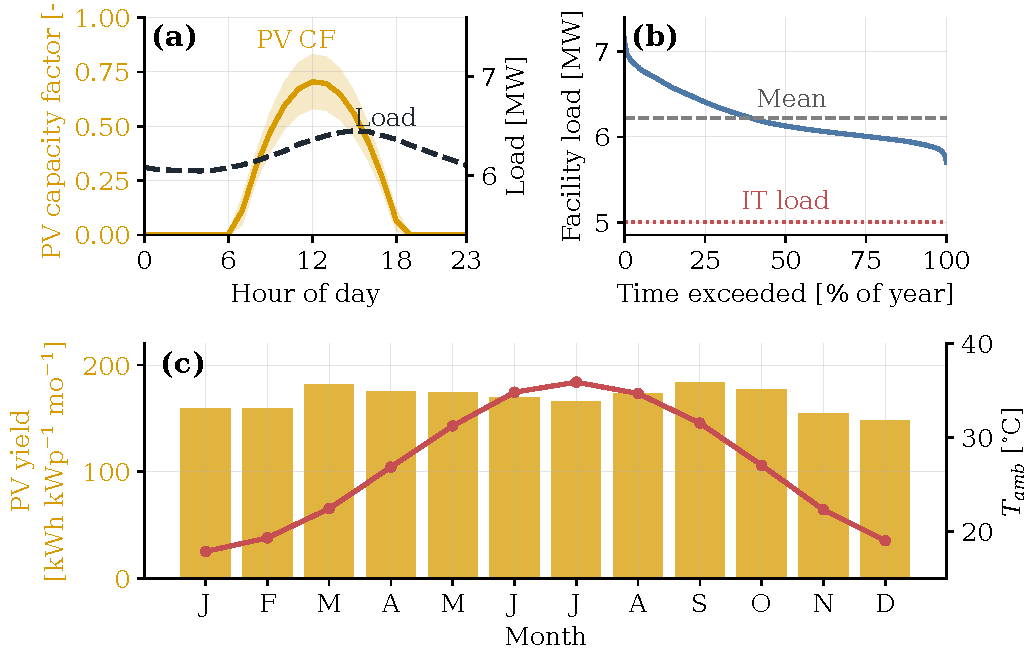
\includegraphics[width=\textwidth]{fig2_resource_load.pdf}
\caption{Resource and load characteristics: (a) mean diurnal PV capacity-factor and facility-load profiles, (b) annual load-duration curve with the 5~MW critical-IT load and 6.224~MW mean total load marked, and (c) monthly PV yield and mean ambient temperature.}
\label{fig:resource}
\end{figure*}

\subsection{Islanded Outage Dispatch}

Islanded dispatch for the selected design (PV~=~22~MW, EZ~=~10~MW, FC~=~5~MW, 57-h/17{,}102-kg tank) is illustrated in Fig.~\ref{fig:outage} for the most H$_2$-demanding event in the 5000-trial set: an 87.19-hour outage requiring 56.95~h of fuel-cell-equivalent hydrogen after direct PV service. The power panel separates the two reliability mechanisms: PV covers daylight critical load, while the fuel cell supplies night-time and low-irradiance deficits up to its 5~MW rating. The tank falls from 100\% to 0.1\%, indicating a reliability-tight design rather than excess storage. The diesel genset is retained for contingency but is not dispatched.

The outage trace also highlights a modelling choice that affects interpretation. Islanded PV surplus is curtailed rather than routed to the electrolyser, so the tank cannot recharge during the event. The selected design is therefore sized for a conservative outage-only reserve policy; allowing islanded electrolysis could reduce curtailment in long sunny outages, but would require additional controls, safety interlocks and operating validation.

\begin{figure*}[!t]
\centering
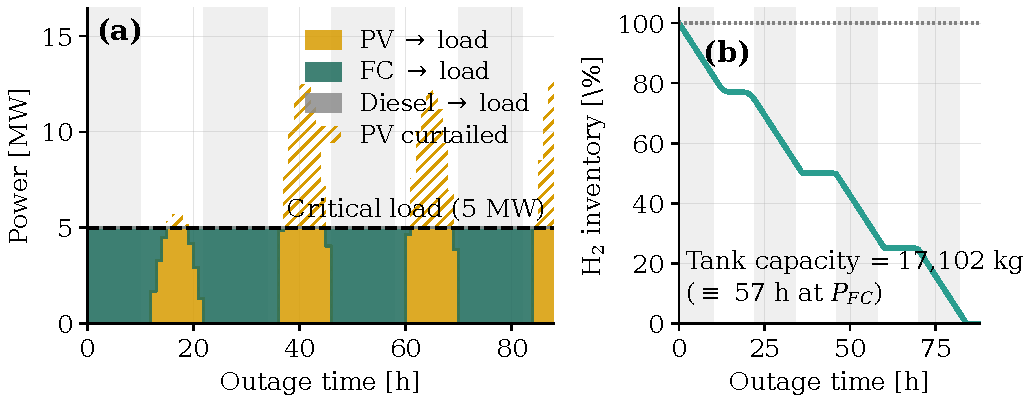
\includegraphics[width=\textwidth]{fig3_outage_dispatch.pdf}
\caption{Example islanded-outage dispatch for the selected PV~=~22~MW, 57-h design, using the most H$_2$-demanding event in the 5000-trial Monte Carlo set. (a) PV and fuel-cell supply to the 5~MW critical load, with curtailed PV surplus hatched. (b) Hydrogen inventory over the same window.}
\label{fig:outage}
\end{figure*}

\subsection{Reliability Landscape: Absence of Saturation}
\label{sec:saturation}

The reliability transition region in Fig.~\ref{fig:heatmap} shows $P_{\mathrm{survive}}(\mathrm{PV}, \mathrm{H_2\ autonomy})$. At zero autonomy, PV alone gives $P_{\mathrm{survive}}=0.085$--0.272 over the refined PV range. With storage, survival rises monotonically: in the displayed window, the transition to $P_{\mathrm{survive}}=1.000$ moves from 59~h at 18~MW to 57~h at 22--24~MW. The printed cell values show that extra PV shifts the threshold only slightly once the tank is large enough. Thus the sampled-set reliability does not exhibit the sub-unity plateau seen in a companion battery-only case, where cycling and power limits cap survival at 0.458.

\begin{figure*}[!t]
\centering
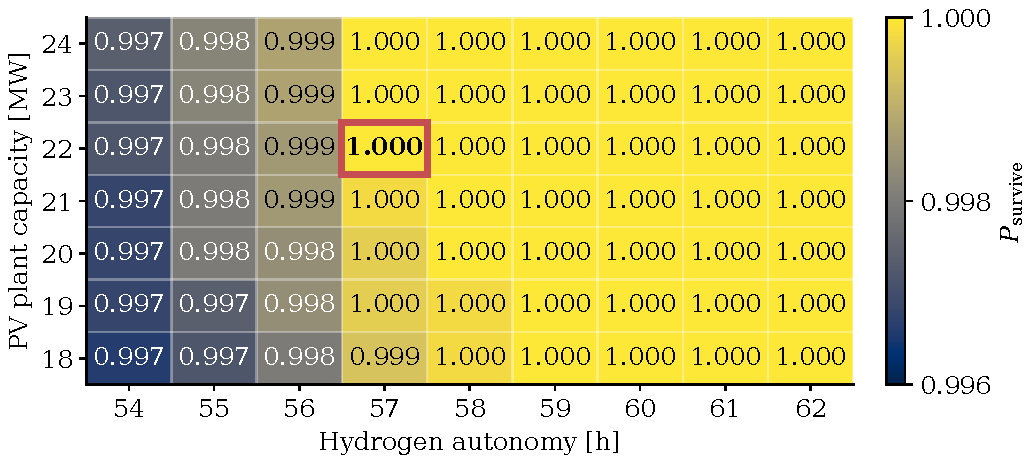
\includegraphics[width=\textwidth]{fig4_reliability_heatmap.pdf}
\caption{Outage Survival Probability $P_{\mathrm{survive}}$ in the reliability-transition window of the refined PV $\times$ H$_2$-autonomy sweep (PV+H$_2$ only, no diesel). Cell values are printed; the orange box marks the selected PV~=~22~MW, 57-h design.}
\label{fig:heatmap}
\end{figure*}

The mechanism is inventory accumulation. A battery cycles daily, so usable depth is rate-limited by its charge/discharge power. The hydrogen tank instead fills over the year and is not cycled down in normal operation; once full, its reliability depends primarily on whether capacity exceeds the sampled outage draw. For the most demanding sampled event in Fig.~\ref{fig:outage}, the 22~MW PV field reduces the tank requirement to 56.95~h of fuel-cell autonomy, explaining why the refined optimiser selects 57~h rather than the coarse-grid 64~h value.

\subsection{Cost-Reliability Pareto Front and Selected Design}
\label{sec:pareto}

The cost-reliability Pareto front in Fig.~\ref{fig:pareto} plots all 2409 configurations in $(P_{\mathrm{survive}}, \mathrm{LCOE})$ space. The grey cloud contains evaluated designs, while the teal curve isolates the non-dominated boundary from a no-storage PV point at $P_{\mathrm{survive}}=0.241$, LCOE~=~0.0635~\$~kWh$^{-1}$, to the selected 22~MW/57~h design at $P_{\mathrm{survive}}=1.000$, LCOE~=~0.1272~\$~kWh$^{-1}$. The selected point is the lowest-cost configuration with zero unmet energy across all 5000 events; its annualised PV+H$_2$+grid cost is \$6.934M~yr$^{-1}$.

From a design-screening perspective, the frontier separates capacity that changes resilience from capacity that only increases cost. Designs below the knee are cheaper but leave sampled diesel energy; designs beyond the selected point add autonomy without changing the outage set. The chosen point should therefore be read as the least-cost sampled-reliable boundary, not as a universal optimum under every tariff, carbon price or outage distribution.

\begin{figure}[!ht]
\centering
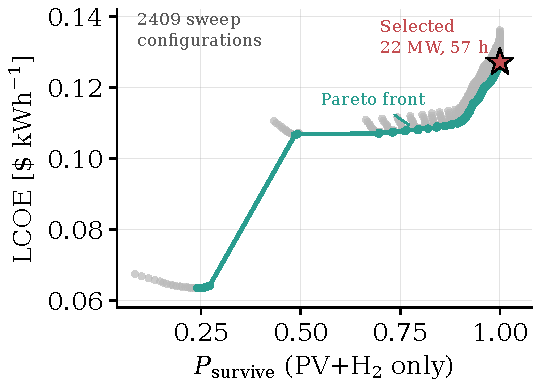
\includegraphics[width=0.92\columnwidth]{fig5_pareto_front.pdf}
\caption{Cost-reliability Pareto front for the refined sweep. Grey points are evaluated designs, the teal curve is the Pareto front, and the star marks the selected PV~=~22~MW, 57-h design at $P_{\mathrm{survive}}=1.000$.}
\label{fig:pareto}
\end{figure}

\subsection{Selected Design versus Grid-Plus-Diesel Baseline}
\label{sec:results-e}

The selected design -- PV~=~22~MW, EZ~=~10~MW, FC~=~5~MW, 57-h tank -- achieves $P_{\mathrm{survive}}=1.000$, $\mathrm{CFE}=0.443$ and $\mathrm{LCOE}=0.1272$~\$~kWh$^{-1}$ before retained-diesel fixed cost. Fig.~\ref{fig:comparison} compares this design plus the same N+1 10~MW genset against the grid-plus-diesel baseline, where the grid serves 54{,}520~MWh~yr$^{-1}$ and the genset supplies $8.175~\mathrm{h}\times2~\mathrm{yr}^{-1}\times5~\mathrm{MW}=81.75$~MWh~yr$^{-1}$ of design-basis outage energy.

\begin{figure}[!ht]
\centering
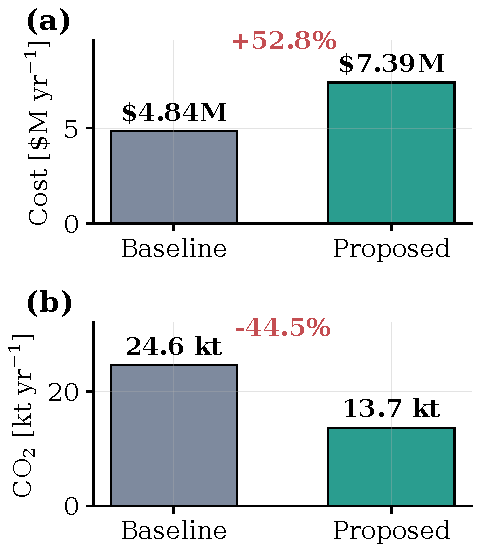
\includegraphics[width=0.92\columnwidth]{fig6_baseline_comparison.pdf}
\caption{Annualised system cost and annual CO$_2$ emissions for the incumbent grid-plus-diesel baseline and the selected PV-H$_2$-plus-diesel design. The same N+1 diesel genset is retained in the proposed design's cost but contributes zero fuel cost or emissions, since it is never dispatched.}
\label{fig:comparison}
\end{figure}

Annualised cost rises from \$4.838M~yr$^{-1}$ to \$7.392M~yr$^{-1}$, a 52.8\% increase, while CO\textsubscript{2} falls from 24.6 to 13.7~kt~yr$^{-1}$ (44.5\% reduction), giving \$233.6~tCO\textsubscript{2}$^{-1}$ abatement. The bar decomposition shows that the premium is driven by the PV-electrolyser-fuel-cell-tank chain, not by retained diesel fixed cost, which is common to both cases. Proposed-system cost comprises PV \$1.663M, electrolyser \$1.492M, fuel cell \$0.839M, hydrogen tank \$1.121M, net grid exchange \$1.819M, and diesel fixed cost \$0.458M~yr$^{-1}$. Since $\mathrm{EUE}_{\mathrm{yr}}=0$, the genset burns no fuel and $f_E=100\%$.

Relative to the companion battery result, hydrogen removes the sampled diesel energy rather than merely reducing it, but at a much larger cost premium. It is therefore a reliability-first option, with the diesel retained for events outside the sampled design envelope.

Across the figures, the design message is consistent. The resource profile defines the PV-surplus window and cooling penalty; the outage dispatch shows the residual night-time tank duty; the heat map locates the 57-h reliability threshold; the Pareto front prices the move to zero sampled unmet energy; and the baseline comparison shows that the result is a decarbonising resilience design, not a least-cost energy-procurement case.

\section{Conclusion}

This study presented a reliability-constrained sizing and dispatch framework for a PV-electrolyser-fuel-cell-H$_2$-grid data-centre microgrid with retained diesel backstop. For a 5~MW Abu Dhabi case, the lowest-cost sampled-reliable design uses 22~MW PV and a 57-hour (17{,}102-kg) tank, achieving $P_{\mathrm{survive}}=1.000$, $\mathrm{CFE}=0.443$ and $\mathrm{LCOE}=0.1272$~\$~kWh$^{-1}$. It cuts CO\textsubscript{2} by 44.5\% at a 52.8\% cost premium, or about \$233.6~tCO\textsubscript{2}$^{-1}$. The central mechanism is annual hydrogen inventory accumulation: survival keeps improving with autonomy until the sampled outage draw is covered. Future work should test hybrid battery-hydrogen sizing, measured outage/weather sequences, multiple climates and electrolyser operation during extended outages.

\bibliographystyle{IEEEtran}
\bibliography{refs}

\end{document}
